\section{Background: {\maas} and Autoscaling}
\label{sec:bg}

\subsection{System setup: model-serving-as-a-service (\maas)}
\label{sec:model}     

\begin{figure*}[!t]
    %\hspace{-3mm}
    \centering
    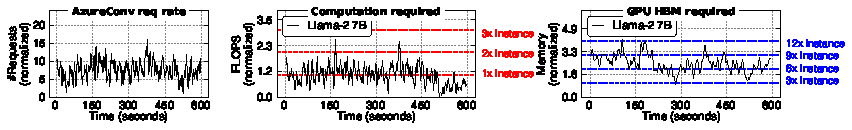
\includegraphics[width=1.01\textwidth,center]{./data/problem/scripts/problem.pdf} \\[0pt]
    \begin{minipage}{1\linewidth}
    \caption{\small{\textit{
        The timeline of request incoming rate of a real-world AzureConv~\cite{AzurePublicDataset} trace (a), 
        its computation (b) and memory requirements 
        (c) when serving this workload without SLO violation. 
    }}}
    \label{fig:problem-statement}
    \end{minipage} \\[-15pt]
\end{figure*} 

\begin{figure}[!t]
    %    \vspace{2mm}
        \begin{minipage}{1\linewidth}
        \hspace{-1mm}
        \centering    
        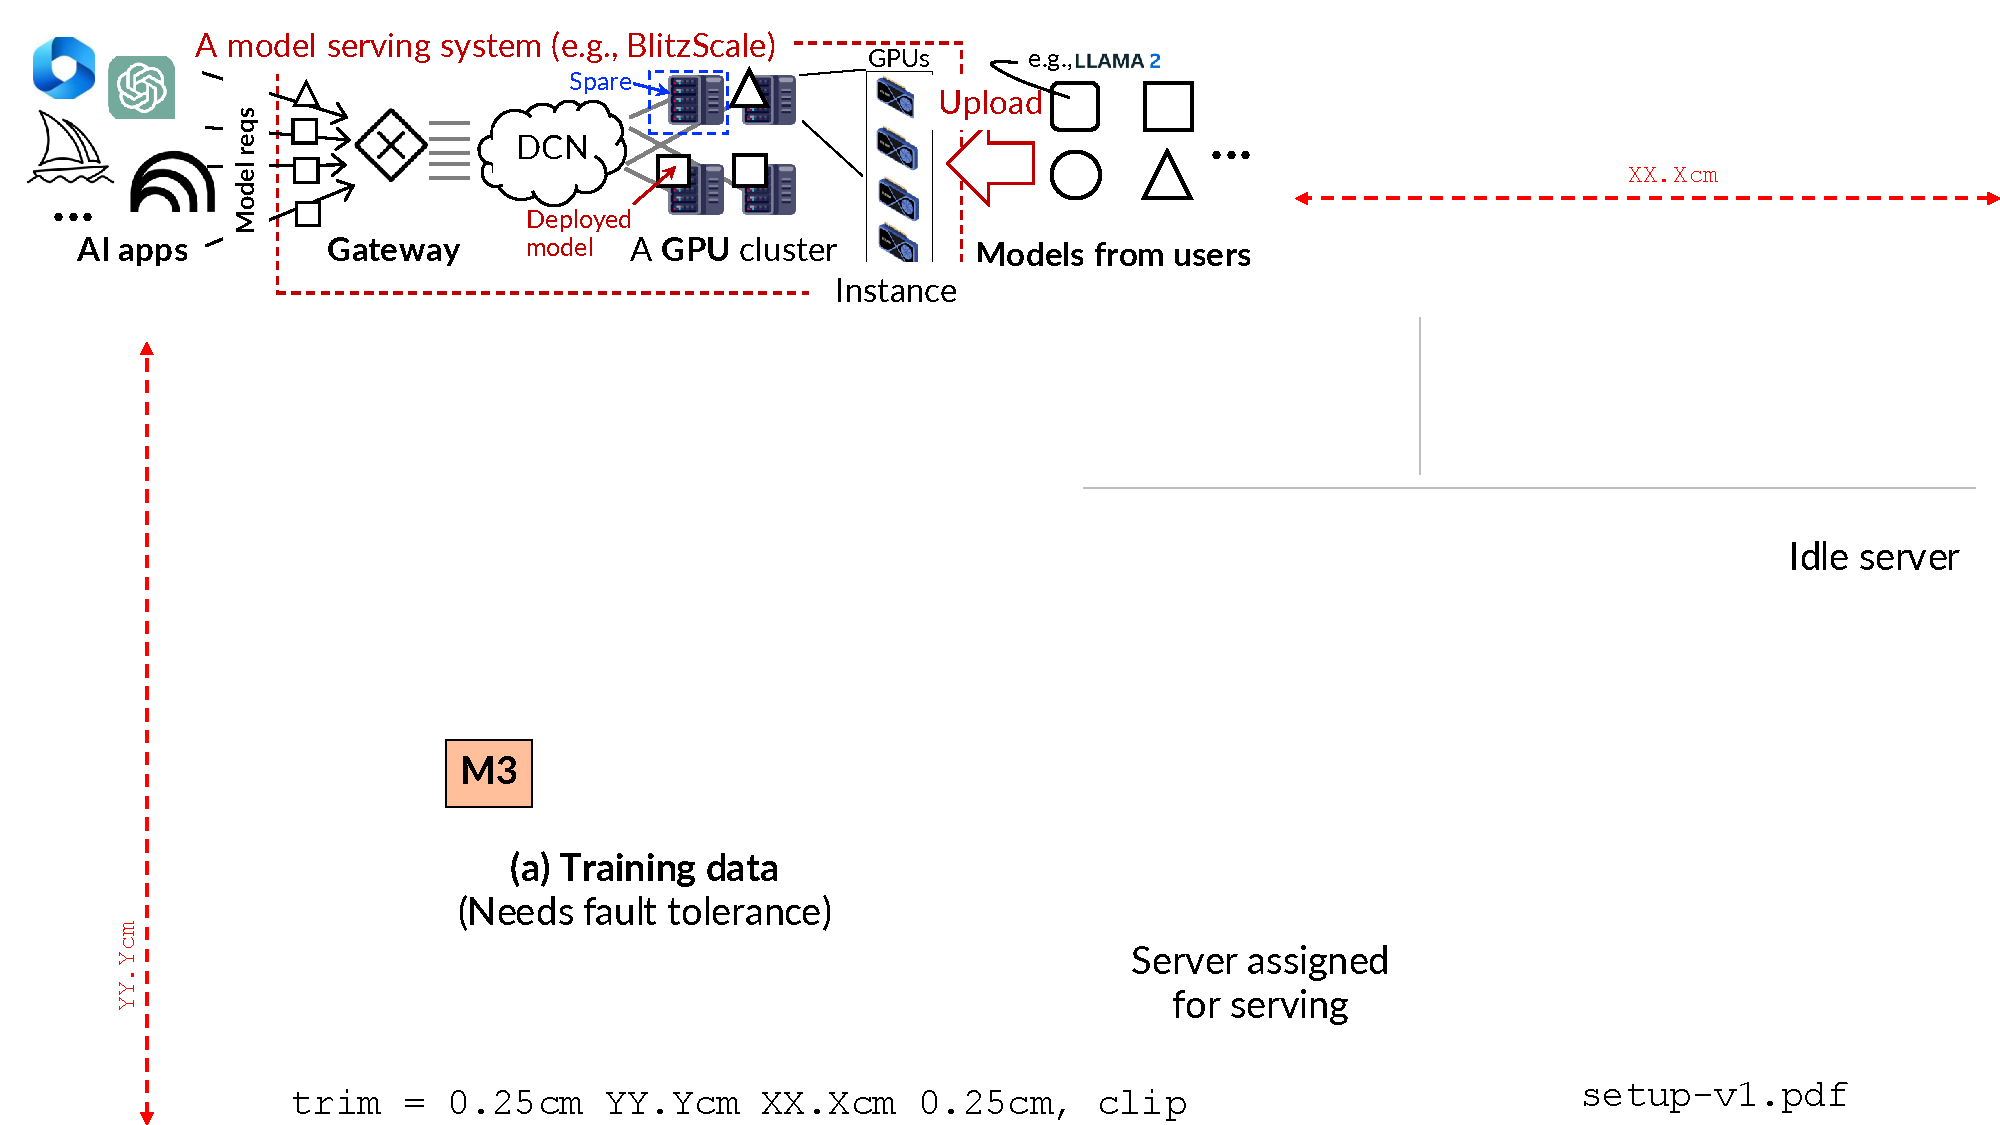
\includegraphics[width=\columnwidth, trim=0.25cm 13.8cm 12cm 0.25cm, clip]{figs/setup-v1.pdf} \\[1pt]
        \end{minipage} \\[3pt]
        \begin{minipage}{1\linewidth}
        \caption{\small{\textit{
            An illustration of Model as a Service ({\maas}) system. 
            DCN states for \uline{d}ata \uline{c}enter \uline{n}etwork. 
        }}}
        \label{fig:setup}
        \end{minipage} \\[-20pt]
        \end{figure} 

\nospacestitle{{\maas} system setup and the serving instance.\,}
{\sys} targets a {\maas} scenario~\cite{serverless-together-ai,serverless-ray,deepinfra,DBLP:conf/asplos/YangZLZLZCL22,ali-serverless-llm,aws-serverless-llm,DBLP:journals/corr/abs-2401-14351}:
the cloud allows the users to deploy their model serving on its managed hardware,
and only charges users based on the number of requests processed within SLO~\cite{aws-serverless-llm,ali-serverless-llm}.
The model can be popular open-source models like Qwen~\cite{qwens}
or customized models uploaded by the users.
Thanks to the above pricing strategy,
the cloud can dynamically adjust hardware resources to a specific model
to maximize its hardware utilization.
{\fig{fig:setup}} shows a typical deployment of a {\maas} system.
For each user-deployed model,
the system dynamically allocates the required hardware resources (GPUs) to serve the
inference requests of the model.
Note that due to the diversity of AI applications,
there would be hundreds or even thousands of models served simultaneously by a {\maas} system~\cite{alibailian}.

In this paper,
we use \emph{instance} to denote a set of GPUs storing
a complete copy of a model parameter for serving this model.
An instance can have a single GPU or multiple GPUs when the parameter
is large and sharded across them, e.g., with tensor parallelism~\cite{narayanan2021efficient}.
Because each instance has a maximal serving throughput,
the cloud can deploy multiply instances of the same model
by provisioning multiple sets of GPUs, 
where the number of instances is dynamically scaled based on the incoming request rate.
{\sys} supports autoscaling with all existing model serving methods at the instance level. 

\stitle{Serving within an instance: non-LLM \& LLM. \,}
Each serving instance processes requests in the following workflow:
it queries the model in a layer-by-layer computation paradigm (see {\fig{fig:overview}} (a))
and gets the final results.
For simple models like vision models,
the model is queried once with the input data (image).
On the other hand, for large language models (LLMs)~\cite{DBLP:conf/nips/VaswaniSPUJGKP17},
the request queries the model multiple times:
the model is first queried with input text (prompt)
to produce a result (token).
This first query is typically termed \emph{prefill}.
The token is then used to generate subsequent tokens iteratively
until the model returns an end-of-sequence token.
The auto-regressive phase is termed \emph{decode}.

We note two important features of LLMs.
First,
the performance for prefill and decode is measured separately.
Prefill is evaluated with the time-to-first-token (TTFT)
while decode is evaluated using time-between-tokens (TBT).
Second, the LLM query is stateful:
the intermediate results---usually termed as \emph{KVCache}---are cached in GPU memory
during the auto-regressive phase of a request for acceleration.

\stitle{Serving across instances:  prefill and decode (PD) disaggregated LLM serving. \,}
Observing the different computing paradigms of prefill and decode,
recent works propose separating the instances for prefill and decode (PD disaggregation)
when processing serving requests~\cite{DBLP:conf/isca/PatelCZSGMB24, DBLP:conf/osdi/ZhongLCHZL0024,DBLP:journals/corr/abs-2401-11181}.
Specifically, for each request, one instance processes the prefill phase (prefill instance )
and another instance (decode instance) processes the decode phase.
This paradigm requires excessive data movement between the two instances
because the prefill instance needs to transfer the KVCache to the decode instance.
{\sys} works for both PD disaggregated and non-disaggregated LLM serving.


\iffalse
For each user-provided model, the system allocates appropriate number of GPUs to serve it.
In our example, model {$\square$} utilizes two machines, while model {$\vartriangle$} uses only one.
\fi

  

\subsection{Dynamic hardware demands when serving a model}
\label{sec:problem-statement}

%\nospacestitle{Unpredictable and fluctuating hardware demands for serving a single model.}
\noindent
Determining the hardware requirements, i.e.,
the right number of instances for serving a model is challenging
because the hardware demands are unpredictable and fluctuating.
First,
the incoming request rate for a serving workload fluctuates over time
and is hard to predict~\cite{DBLP:journals/corr/abs-2401-14351,DBLP:conf/usenix/ShahradFGCBCLTR20,DBLP:conf/nsdi/0025TKS23}.
{\fig{fig:problem-statement}} (a) presents the number of requests sent to a single model service
over time from a real-world trace---BurstGPT~\cite{wang2024burstgpt}:
the incoming inference requests increase 5\,$\times$ within 2 seconds with no predictable trend.
Since the FLOPS of an instance is fixed, 
the unpredictable rate causes 
the computation requirement---FLOPS required to finish the pending
requests within SLO---unpredictable.
{\fig{fig:problem-statement}} (b) confirms this by measuring the requirement 
of the prefill instances when serving the BurstGPT with Llama2-7B.

Second,
serving modern models like LLM
has non-trivial and unpredictable memory requirements.
As shown in
{\fig{fig:problem-statement}} (c),
the KVCache usage of the decode instances is multiple times larger than the memory capacity
of a single instance and fluctuates over time (3--12\,$\times$) when serving the BurstGPT workload with Llama2-7B.
The root cause is that
the KVCache of requests must be stationary in GPU memory during the decode phase.
The KVCache of requests are large, e.g., 190--760\,GB for Llama2-7B to serve BurstGPT, 
and the stay time is unpredictable due to the auto-regressive nature of LLMs.
To avoid performance losses when out of memory,
a {\maas} system must provision sufficient instances
to hold KVCache from ongoing requests,
so the number of instances required by a model also unpredictably fluctuates.


\subsection{Model autoscaling for handling dynamic demands}

\noindent
Model autoscaling, which dynamically deploys\footnote{\footnotesize{It also stops a serving instance to scale down.
Since scaling down is simpler, we omit its details for brevity.}}
serving instances on spare GPUs to scale up the serving capability, is
a promising solution to handle fluctuated and unpredictable computation and memory demands~\cite{DBLP:journals/corr/abs-2401-14351,DBLP:conf/asplos/YangZLZLZCL22,serverless-ray}.
The rationale is that though a single model's workload is unpredictable,
the aggregated workloads of all models served by a platform are relatively stable~\cite{DBLP:conf/nsdi/0025TKS23}.
Thus, when the load of a specific model service increases,
we are able to find spare GPUs from other models to scale up the serving capability of this model. 

Autoscaling an instance requires two basic steps:
(1) initialize a proper execution context, e.g., create CUDA contexts (control plane)
and 
(2) load the model parameters to the GPUs' memory (data plane). 
We focus on (2) because (1) can be minimized with recent advances
in GPU startup methods like checkpoint
and restore~\cite{DBLP:journals/corr/abs-2405-12079,DBLP:conf/asplos/ZengXGCL25} 
and our Rust/C++-based serving platform
(see also \textsection{\ref{sec:eval-ablation}}).
For (2), the state-of-the-art system---ServerlessLLM~\cite{DBLP:journals/corr/abs-2401-14351}
optimizes the data plane with SSD-optimized parameter loading.
Unfortunately, it does not account for the scaling speed required by models.
Our measurements in the next section
show that SSD-based scaling significantly lags behind applications' requirements.


\begin{figure*}[!t]
    %\hspace{-3mm}
    \centering
    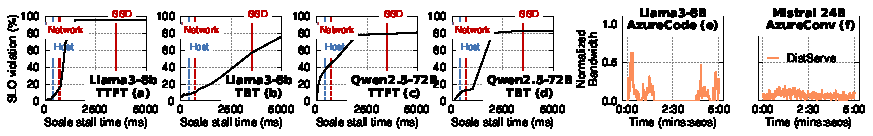
\includegraphics[width=1.01\textwidth,center]{./data/motiv-slo-all.pdf} \\[2pt]
    \begin{minipage}{1\linewidth}
    \caption{\small{\textit{
        A characterization of SLO attainment for different inference cases (a)--(d)
        with varied duration of autoscaling stops on BurstGPT~\cite{wang2024burstgpt}. 
        (e) and (f): an analysis of compute network usage in serving workloads.
        The evaluation setup is in \textsection{\ref{sec:eval}}.
    }}}
    \label{fig:motiv-scale-speed}
    \end{minipage} \\[-5pt]
\end{figure*}

\section{Characterizing Scaling Requirements and Compute Network between Instances}
\label{sec:bg-motiv}  

\nospacestitle{Model autoscaling requires fast data plane. \,}
%A key system requirement is fast scaling speed,
%i.e., how fast the scaled instance can improve a model's serving throughput.
If the data plane speed is not fast enough, during burst period, the requests
still violate the SLO due to increased queueing time.
Specifically, SLO defines the tolerable end-to-end latency measured from the 
time a request is sent to the system to the time the inference response is returned.
Thus, the latency includes the queueing delays waiting for the scaled instance 
to be ready for inference.


%We conducted our experiment using an optimized version of DistServe~\cite{DBLP:conf/osdi/ZhongLCHZL0024}, 
%that supports the state-of-the-art autoscaling policy (described in \textsection{\ref{sec:design-others}}).  
%DistServe disaggregates the instances for prefilling and decoding, 
%allowing us to precisely measure the SLO violations of TTFT and TBT. 
To characterize how different scaling speeds affect SLO attainments,
we implemented a simulator on DistServe~\cite{DBLP:conf/osdi/ZhongLCHZL0024}
that provisions models to all GPUs and applies manual delays
based on the simulated speed for modeling different scaling speeds.
We set TTFT and TBT SLO based on inference speed of different models following
prior works~\cite{DBLP:conf/osdi/ZhongLCHZL0024}.
Specifically, we use 450\,ms and 150\,ms for Llama3-8B model,
and 1250\,ms and 200\,ms for Qwen2.5-72B model with tensor parallelism degree of 4.
\textsection{\ref{sec:eval}} describes the detailed evaluation setup.

{\fig{fig:motiv-scale-speed}} (a)--(d) shows the results: 
We can see that 
for a 72\,B model,
maintaining SLO violations below 60\,\%
requires a minimum per-instance scaling speed of 220\,Gbps per-GPU\footnote{\footnotesize{72\,B model uses four GPUs per-instance.}},
which is only achievable when the model parameters are loaded from the host memory.
The scaling time requirement correlates directly with inference time---our evaluated workload (BurstGPT~\cite{wang2024burstgpt})
has an average TTFT of 771\,ms (with queueing time).
Thus, to achieve 1250\,ms SLO for all requests,
the scale time must be below 500\,ms,
so a 576\,Gbps per-GPU network speed
is required (measured by dividing the parameter size by the scale time).
This far exceeds what vendor-provided per-GPU
SSDs bandwidth can deliver (2--10\,Gbps per-GPU~\cite{googleinstance,awsinstance,volcanoinstance}, 
detailed in \textsection{\ref{sec:appendix-hardware}}).

\begin{figure}[!t]
    %\hspace{-3mm}
    \centering
    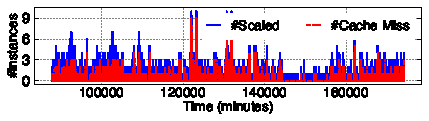
\includegraphics[width=1.01\linewidth,center]{./data/motiv-cache-miss.pdf} \\[1pt]
    \begin{minipage}{1\linewidth}
    \caption{\textit{\small{
        An analysis of host cache misses when running ServerlessLLM~\cite{DBLP:journals/corr/abs-2401-14351}
        on BurstGPT~\cite{wang2024burstgpt}.
    }}}
    \label{fig:motiv-cache-miss}
    \end{minipage} \\[-5pt]
\end{figure} 

\stitle{Loading model parameters from host memory is not effective due to misses. \,}
While caching the parameters on the host CPU memory 
can meet the scaling speed requirement for some setups (e.g., 8\,B, 24\,B)
with the fast host-GPU interconnects (256\,Gbps PCIe 4.0),
cache misses are common in real-world traces,
because the scarce host memory cannot support the caching all models deployed on the {\maas}. 
{\fig{fig:motiv-cache-miss}} presents the number of instances scaled and cache misses 
encountered in the BurstGPT 
workload using ServerlessLLM~\cite{DBLP:journals/corr/abs-2401-14351}. 
Following its setup,
we set a 5-minute keep-alive interval for caching models at the host. 
The miss rates range from 20--46\%, 
depending on the time, 
which aligns with the numbers reported in ServerlessLLM's paper (25--60\%).  
Interestingly, many misses occur when scaling multiple instances, 
because involving more hosts increases the probability of scaling 
a model on a host without the cached parameters.
Therefore, we still need accelerating scaling speed when the model parameters
are not cached at the host.

\begin{figure}[!t]
    %    \vspace{2mm}
        \begin{minipage}{1\linewidth}
        \hspace{-1mm}
        \centering    
        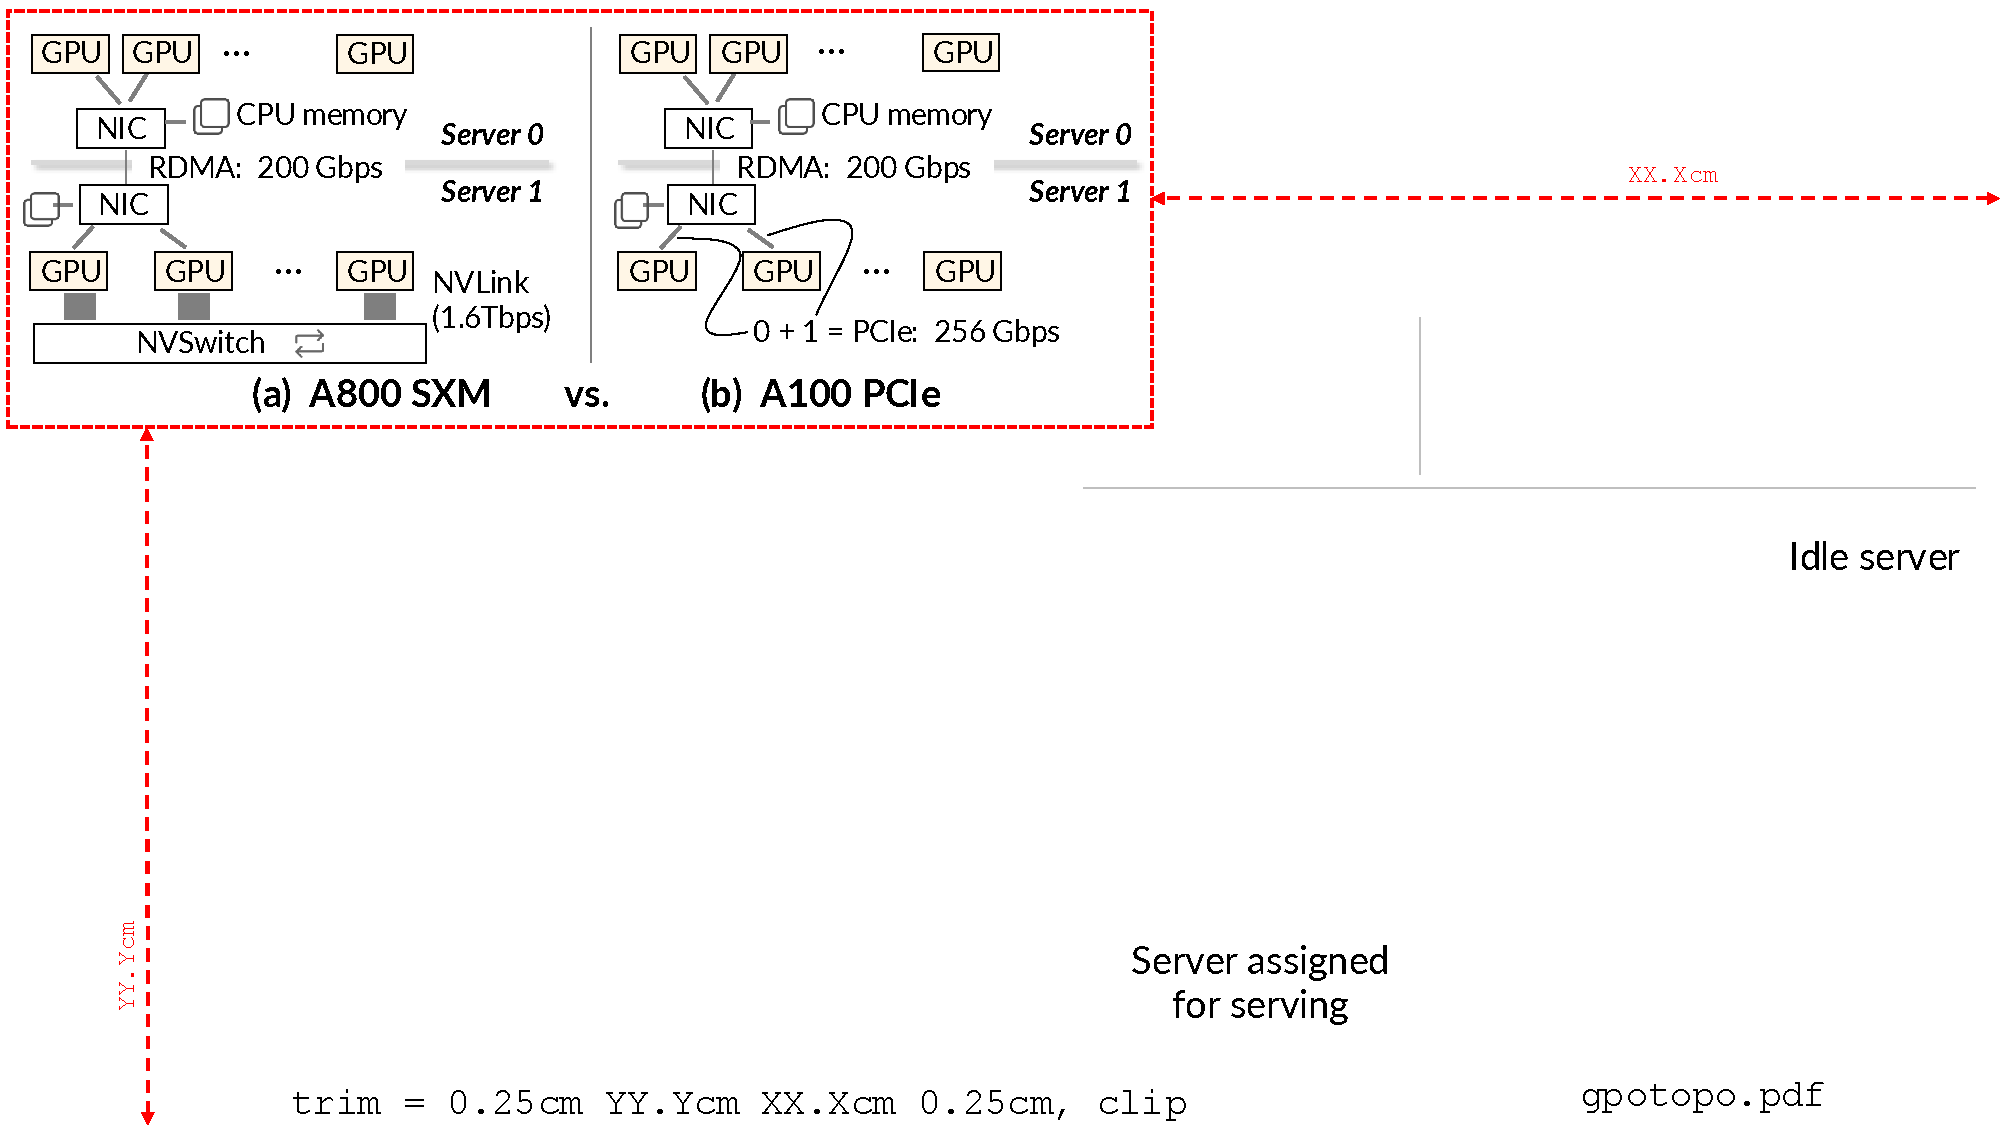
\includegraphics[width=.99\textwidth, trim=0.25cm 11.9cm 14.4cm 0.25cm, clip]{figs/gputopo.pdf} \\[1pt]
        \end{minipage} \\[4pt]
        \begin{minipage}{1\linewidth}
            \caption{\textit{\small{
            A illustration of networking in {\maas} with NVLink (a) and without it. 
            Note that the 256\,Gbps PCIe is shared between two GPUs attached to it~\cite{nvidia-all-to-all}.
        }}}
        \label{fig:gputopo}
        \end{minipage} \\[-10pt]
        \end{figure}        


\stitle{Opportunity: fast and underutilized compute network. \,}
First, compute networks  between GPUs (and CPUs) have comparable or even faster speeds
than host-to-GPU link. As shown in {\fig{fig:gputopo}},
the inter-GPU network (RDMA) operates at 200\,Gbps,
which is close to the host-to-GPU PCIe speed (256\,Gbps). 
With NVLink, the speed is much faster. 
More importantly, these networks are underutilized during serving.
{\fig{fig:motiv-scale-speed}} (e) and (f) measure the peak
network usage of DistServe~\cite{DBLP:conf/osdi/ZhongLCHZL0024},
a PD disaggregated serving system that heavily utilizes the network due to KVCache transfers.
To measure peak usage, we provisioned all the GPUs for serving,
and evaluate a workload with the maximal request rate that our clusters can serve.
Even under peak load, more than 40\% of the network capacity is free,
opening up the opportunity to use the compute network for the scaling data plane.